\documentclass[UTF8,fontset=ubuntu]{ctexart}
\usepackage{graphicx}
\begin{document}
\parindent=0cm
netstat - 打印网络连接/路由表/接口统计/伪装连接/多播成员。包含在net-tools工具包中\\[1ex]

语法\\
netstat [option]\\[1ex]

参数释义\\
\qquad 当前开放的套接口信息

--route, -r\quad 路由表信息

--groups, -g\quad 多播组成员信息

--interfaces, -i\quad 网卡接口信息

--masquerade, -M\quad 伪装连接信息

--statistics, -s\quad 各种协议的汇总信息

--numeric, -n\quad 显示数字形式的主机/端口/用户名

--numeric-hosts\quad 显示数字形式的主机名,不影响端口和用户名解析

--numeric-ports\quad 显示数字形式的端口,不影响主机和用户名解析

--numeric-users\quad 显示数字形式用户名(userID),不影响主机和端口解析

--protocol=\textless family \textgreater, -A\quad IP层协议族。如IPv4-inet,IPv6-inet6

--continuous, -c\quad 每秒都进行信息的连续打印

--extend, -e\quad 显示额外的信息。User和Inode信息

--timers, -o\quad 网络计时器信息。其中,第一列代表计时器类型,第二列代表对应的时间值。列表如下:
    
\qquad 第一列:\par
\qquad keeplive - keeplive时间计时器\par
\qquad on - 重发时间计时\par
\qquad timewait - 等待时间计时\par
\qquad off - 没有时间计时
    
\qquad 第二列(a/b/c):\par
\qquad a - 计与第一列的对应关系如下:\par
\qquad\qquad keeplive - keeplive时间,由tcp\_keeplive\_time确定\par
\qquad\qquad on - 重发时间\par
\qquad\qquad timewait - 等待时间\par
\qquad b - 已经重发的次数\par
\qquad c - keeplive已发送的probe探测包次数,由tcp\_keeplive\_probes决定上限\par
    
\qquad keeplive原理:\par
\qquad 1.在tcp\_keeplive\_time时间内,如果期间发送数据互通,则重置到该值进行倒数;如超过该时间无数据互通,则进入probe探测包发送\par
\qquad 2.probe探测包总共发射次数由tcp\_keeplive\_probes决定,并且发送时间间隔由tcp\_keeplive\_intvl决定\par

--programs, -p\quad 套接字所属进程的PID和名称

--listening, -l\quad 只显示正在侦听的套接字

--all, -a\quad 显示所有正在或不在侦听的套接字

-F\quad 显示FIB的路由信息

-C\quad 显示路由缓存信息\\[1ex]


TCP连接状态:\\
ESTABLISHED - 套接字的有效连接

SYN\_SENT - 套接字尝试建立连接

SYN\_RECV - 套接字接收到连接请求

FIN\_WAIT1 - 主动结束方第一次发送FIN后的状态

FIN\_WAIT2 - 主动结束方第一次收到ACK后的状态

TIME\_WAIT - 主动结束方第一次接收到FIN后的状态

CLOSED - 套接字连接已被关闭

CLOSE\_WAIT - 被动结束方第一次接收到FIN后的状态
 
LASTi\_ACK - 被动结束方第一次发送FIN后的状态

LISTEN - 套接字侦听连接。需要指定-l或-a参数

CLOSING - 套接字都已关闭,但还未把所有数据发出

UNKNOWN - 套接字状态未知
\begin{figure}
	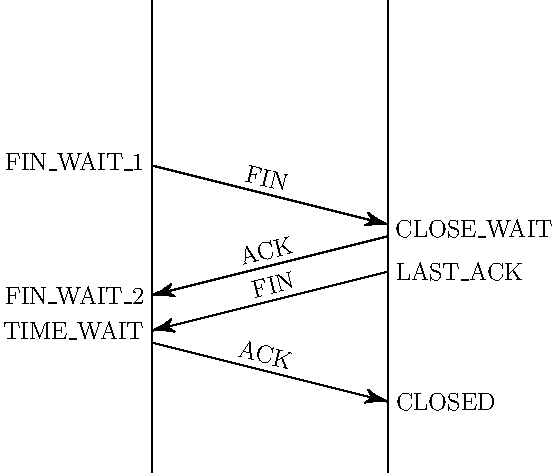
\includegraphics{four_handshake.pdf}
	\caption{四次握手图解}
\end{figure}
\end{document}
